\let\negmedspace\undefined
\let\negthickspace\undefined
\documentclass[journal]{IEEEtran}
\usepackage[a5paper, margin=10mm, onecolumn]{geometry}
%\usepackage{lmodern} % Ensure lmodern is loaded for pdflatex
\usepackage{tfrupee} % Include tfrupee package

\setlength{\headheight}{1cm} % Set the height of the header box
\setlength{\headsep}{0mm}     % Set the distance between the header box and the top of the text

\usepackage{gvv-book}
\usepackage{gvv}
\usepackage{cite}
\usepackage{amsmath,amssymb,amsfonts,amsthm}
\usepackage{algorithmic}
\usepackage{graphicx}
\usepackage{textcomp}
\usepackage{xcolor}
\usepackage{txfonts}
\usepackage{listings}
\usepackage{enumitem}
\usepackage{mathtools}
\usepackage{gensymb}
\usepackage{comment}
\usepackage[breaklinks=true]{hyperref}
\usepackage{tkz-euclide} 
\usepackage{listings}
% \usepackage{gvv}                                        
\def\inputGnumericTable{}                                 
\usepackage[latin1]{inputenc}                                
\usepackage{color}                                            
\usepackage{array}                                            
\usepackage{longtable}                                       
\usepackage{calc}                                             
\usepackage{multirow}                                         
\usepackage{hhline}                                           
\usepackage{ifthen}                                           
\usepackage{lscape}
\usepackage{circuitikz}
\tikzstyle{block} = [rectangle, draw, fill=blue!20, 
    text width=4em, text centered, rounded corners, minimum height=3em]
\tikzstyle{sum} = [draw, fill=blue!10, circle, minimum size=1cm, node distance=1.5cm]
\tikzstyle{input} = [coordinate]
\tikzstyle{output} = [coordinate]


\begin{document}

\bibliographystyle{IEEEtran}
\vspace{3cm}

\title{2.3.2}
\author{AI25BTECH11039-Harichandana Varanasi}
 \maketitle
% \newpage
% \bigskip
{\let\newpage\relax\maketitle}

\renewcommand{\thefigure}{\theenumi}
\renewcommand{\thetable}{\theenumi}
\setlength{\intextsep}{10pt} % Space between text and floats


\numberwithin{equation}{enumi}
\numberwithin{figure}{enumi}
\renewcommand{\thetable}{\theenumi}



\date{}

\begin{document}
\maketitle


\section*{Question}
\textbf{Q.}\; Find the angle between unit vectors $\vec a$ and $\vec b$ such that $\sqrt{3}\,\vec a-\vec b$ is also a unit vector.


\section*{Solution}
\textbf{Given:} $\|\vec{a}\|=\|\vec{b}\|=1$ and $\bigl\|\sqrt{3}\,\vec{a}-\vec{b}\bigr\|=1$.

\medskip
Use the length definition $\|x\|^2=x^\top x$ and the scalar–product relation $\vec{a}^\top\vec{b}=\|\vec{a}\|\,\|\vec{b}\|\cos\theta$.

\medskip
\[
\begin{aligned}
1
&=\bigl\|\sqrt{3}\,\vec{a}-\vec{b}\bigr\|^{2}\\
&=(\sqrt{3}\,\vec{a}-\vec{b})^\top(\sqrt{3}\,\vec{a}-\vec{b})\\
&=3\,\vec{a}^\top\vec{a}+\vec{b}^\top\vec{b}-2\sqrt{3}\,\vec{a}^\top\vec{b}\\
&=3\cdot 1+1\cdot 1-2\sqrt{3}\,\cos\theta\\
&=4-2\sqrt{3}\,\cos\theta.
\end{aligned}
\]
Hence $\,2\sqrt{3}\,\cos\theta=3\,$, so $\displaystyle \cos\theta=\frac{\sqrt{3}}{2}\,$ and therefore $\boxed{\theta=30^\circ}$.



   \begin{figure}[h!]
\centering
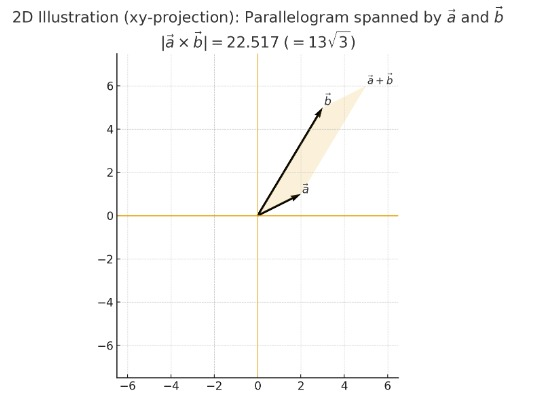
\includegraphics[width=0.7\linewidth]{figs/matgeo2.3.2.jpeg}
\caption{xy-projection of $\vec a$ and $\vec b$; $|\vec a\times\vec b|=13\sqrt{3}$.}

\end{figure} 

\end{document}
